% !TEX TS-program = pdflatex
\documentclass[aspectratio=169]{beamer}
\usetheme{Madrid}
\usecolortheme{default}
\usepackage{booktabs}
\usepackage{pgfplots}
\pgfplotsset{compat=1.17}
\setbeamertemplate{navigation symbols}{}
\setbeamertemplate{footline}[frame number]

\title{Running LatentMAS in one engine}
\subtitle{All of LatentMAS inside a modified vLLM $\cdot$ Qwen3-14B $\cdot$ one H200}
\author{Sagnik Biswas}
\date{29 October 2026}

\begin{document}

\begin{frame}
\titlepage
\end{frame}

\begin{frame}{How LatentMAS runs today}

LatentMAS is four copies of the same model working on one question.
Three helpers ``think silently'' for a few steps; the fourth, the Judger, reads those thoughts and writes the answer.

\vspace{0.5em}
The authors run this in two separate programs:
\begin{itemize}
  \item A research library (Hugging Face) does the silent thinking.
    It is easy to modify but slow, and handles one batch at a time.
  \item A fast serving program (vLLM) writes the Judger's answer.
  \item So the model is loaded into memory \textbf{twice}, and the thoughts
    are handed from one program to the other and re-read.
\end{itemize}

\vspace{0.5em}
vLLM does not support silent thinking out of the box. The authors' README says they modified
parts of vLLM for this; that change is not in their public code.

\end{frame}

\begin{frame}{What we built}

A modified copy of vLLM that does \textbf{all} of LatentMAS by itself.

\begin{itemize}
  \item New mode: instead of picking the next word, the model feeds its own
    internal state back in as the next input. That is the silent thinking.
  \item Each helper's instructions are added to the same running request,
    so the Judger picks up exactly where the helpers left off.
  \item One copy of the model in memory, no hand-off, no re-reading.
  \item Many questions can be processed side by side, including the silent thinking.
  \item If memory runs out and a question gets paused, its silent thoughts are
    saved so it can resume correctly. We tested this on purpose.
\end{itemize}

\end{frame}

\begin{frame}{Grade-school math, one question at a time}

Qwen3-14B, 50 GSM8K questions (the two-program version ran the first 30). Time is the typical (middle) value.

\begin{center}
\begin{tabular}{lrrr}
\toprule
how it was run & correct & time per question & words per second \\
\midrule
Paper's way (research library only) & 49/50 & 13.3 s & 24 \\
Authors' two-program version & 30/30 & 5.1 s & 56 \\
\textbf{Ours (one engine)} & \textbf{49/50} & \textbf{6.0 s} & \textbf{86} \\
Plain model, no helpers & 49/50 & 6.5 s & 68 \\
\bottomrule
\end{tabular}
\end{center}

\begin{itemize}
  \item Same accuracy as the paper's setup.
  \item Ours writes 3.5$\times$ faster than the paper's way, and faster than either alternative.
\end{itemize}

{\footnotesize ``Words'' throughout means the word pieces the model writes, roughly three quarters of an English word each.}

\end{frame}

\begin{frame}{Many questions at once}

Same 50 math questions, sent in groups. Total words written per second, our engine:

\begin{center}
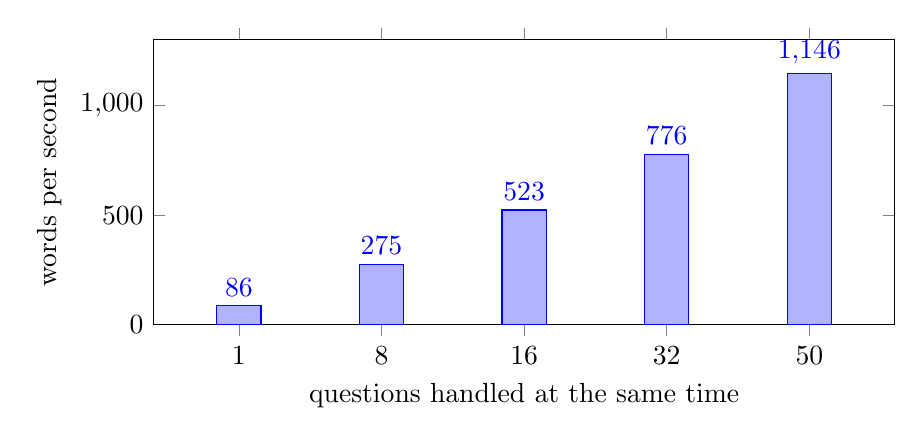
\begin{tikzpicture}
\begin{axis}[
  ybar, bar width=16pt, width=11cm, height=5.2cm,
  symbolic x coords={1,8,16,32,50},
  xtick=data, ymin=0, ymax=1300,
  xlabel={questions handled at the same time},
  ylabel={words per second},
  nodes near coords, nodes near coords align={vertical},
  enlarge x limits=0.15]
\addplot coordinates {(1,86) (8,275) (16,523) (32,776) (50,1146)};
\end{axis}
\end{tikzpicture}
\end{center}

13$\times$ more output per second when all 50 run together, with 49/50 still correct.
The paper's setup cannot do this at all.

\end{frame}

\begin{frame}{Memory}

\begin{center}
\begin{tabular}{lr}
\toprule
how it was run & GPU memory used \\
\midrule
Authors' two-program version & 91 GB \\
\textbf{Ours (one engine)} & \textbf{63 GB} \\
\bottomrule
\end{tabular}
\end{center}

\begin{itemize}
  \item The difference is mostly the second copy of the model (about 28 GB) that we no longer load.
  \item That memory can go to serving more questions at once instead.
\end{itemize}

\end{frame}

\begin{frame}{Summary}

\begin{itemize}
  \item All of LatentMAS now runs inside one fast engine, with one copy of the model.
  \item Same accuracy on grade-school math as the paper's setup.
  \item 3.5$\times$ faster writing one question at a time.
  \item 13$\times$ more output per second with 50 questions at once.
  \item About 28 GB less memory than the authors' two-program version.
\end{itemize}

\end{frame}

\end{document}
